\documentclass[a4paper,11pt]{article}
% \usepackage{fullpage}
% \usepackage[top=2cm, bottom=2cm, left=2cm, right=2cm]{geometry}
\usepackage[margin=2cm]{geometry}
\usepackage[charter]{mathdesign}
\usepackage{epsfig}
\usepackage{graphicx}
% \usepackage{amssymb}
% \usepackage{amsmath}
\usepackage{verbatim}
\usepackage{fancyhdr}
\usepackage{pifont}% http://ctan.org/pkg/pifont
\usepackage[rgb]{xcolor}
\usepackage{tikz}
\usetikzlibrary{matrix,positioning,fit,shapes,arrows,shadows,calc,backgrounds}
\usepackage{pgfplots}
\usepackage{natbib}
\usepackage{enumitem}
\usepackage{pgfgantt}
\usepackage{booktabs}
\usepackage{url}
\usepackage{xspace}
\usepackage{wrapfig}
\usepackage[show]{chato-notes}
\usepackage{multirow}
\usepackage[official]{eurosym}
\usepackage[bottom]{footmisc}

\usepackage{lipsum}% http://ctan.org/pkg/{graphicx,lipsum}
\newcommand{\PRLsep}{\noindent\makebox[\linewidth]{\resizebox{0.3333\linewidth}{1pt}{$\bullet$}}\bigskip}

\definecolor{verylightmagenta}{rgb}{0.95,0.96,1.0}
\definecolor{brightred}{rgb}{0.90,0.2,0.2}

\newcommand{\ag}[1]{\noindent{\color{olive}{\textbf{AG:} #1}}}
% \newcommand{\ag}[1]{}
\newcommand{\instructions}[1]{\noindent{\color{blue}{#1}}}
% \newcommand{\instructions}[1]{}

\newcommand{\mpara}[1]{\medskip\noindent{\bf #1}}
\newcommand{\spara}[1]{\smallskip\noindent{\bf #1}}
\newcommand{\para}[1]{\noindent{\bf #1}}

\newcommand{\acronym}{{\sf\small E\ensuremath{x}CLUS}\xspace}
\newcommand{\acronymtitle}{{\sf\large E\ensuremath{x}CLUS}\xspace}

\newcommand{\rto}{{RT1}\xspace}
\newcommand{\rtw}{{RT2}\xspace}
\newcommand{\rth}{{RT3}\xspace}


\newcommand{\newmodels}{{Novel explainable models}}
\newcommand{\clusterings}{{Beyond centroid-based clustering}}
\newcommand{\covariates}{{Covariate explanations}}

\newcommand{\posthoc}{{\sc PostHoc}}
\newcommand{\joint}{{\sc Joint}}


\newcommand{\proposaltitle}{{Advances in explainable clustering}}
\newcommand{\proposalabstitle}{{Advances in explainable clustering}}

\newcommand{\NP}{{\ensuremath{\mathbf{NP}}}}


%% squishlist
\newcommand{\squishlist}{\begin{list}{$\bullet$}
  { \setlength{\itemsep}{-1pt}
     \setlength{\parsep}{2pt}
     \setlength{\topsep}{2pt}
     \setlength{\partopsep}{0pt}
     \setlength{\leftmargin}{1.5em}
     \setlength{\labelwidth}{1em}
     \setlength{\labelsep}{0.5em} } }
\newcommand{\squishend}{
\end{list}  }


%% gantt stuff

% \definecolor{foobarblue}{RGB}{0,153,255}
% \definecolor{foobaryellow}{RGB}{234,187,0}
% \newganttchartelement{foobar}{
%     foobar/.style={
%         shape=rounded rectangle,
%         inner sep=0pt,
%         draw=foobarblue!50!black,
%         very thick,
%         top color=white,
%         bottom color=foobarblue!50
%     },
%     foobar incomplete/.style={
%         /pgfgantt/foobar,
%         draw=foobaryellow,
%         bottom color=foobaryellow!50
%     },
%     foobar label font=\slshape,
%     foobar left shift=-.1,
%     foobar right shift=.1
% }

%% tikz stuff

\pgfdeclarelayer{background}
\pgfdeclarelayer{foreground}
\pgfsetlayers{background,main,foreground}


\makeatletter
\tikzset{multicircle/.style  args={#1, #2}{%
 alias=tmp@name, % 
  postaction={%
    insert path={
     \pgfextra{% 
     \pgfpointdiff{\pgfpointanchor{\pgf@node@name}{center}}%
                  {\pgfpointanchor{\pgf@node@name}{east}}%            
     \pgfmathsetmacro\insiderad{\pgf@x}%
     %\foreach \c [count=\ci from = 0, evaluate=\ci as \angle using 360 - (\ci) * #1] in {#2}%
        \fill[white] (\pgf@node@name.center)  circle (\insiderad-\pgflinewidth);%
        \draw[#2] (\pgf@node@name.center)  circle (\insiderad-\pgflinewidth);%
        \fill[#2] (\pgf@node@name.center)  -- ++(0:\insiderad-\pgflinewidth) arc (0:#1:\insiderad-\pgflinewidth)--cycle;%
        }}}}}
\makeatother

\definecolor{yafaxiscolor}{rgb}{0.3, 0.3, 0.3}
\definecolor{yafcolor1}{rgb}{0.4, 0.165, 0.553}
\definecolor{yafcolor2}{rgb}{0.949, 0.482, 0.216}
\definecolor{yafcolor3}{rgb}{0.47, 0.549, 0.306}
\definecolor{yafcolor4}{rgb}{0.925, 0.165, 0.224}
\definecolor{yafcolor5}{rgb}{0.141, 0.345, 0.643}
\definecolor{yafcolor6}{rgb}{0.965, 0.933, 0.267}
\definecolor{yafcolor7}{rgb}{0.627, 0.118, 0.165}
\definecolor{yafcolor8}{rgb}{0.878, 0.475, 0.686}
\definecolor{yafcolor9}{rgb}{0.965, 0.733, 0.767}

\newlength{\yafaxispad}
\setlength{\yafaxispad}{-4pt}
\newlength{\yaftlpad}
\setlength{\yaftlpad}{\yafaxispad}
\addtolength{\yaftlpad}{-0pt}
\newlength{\yaflabelpad}
\setlength{\yaflabelpad}{-2pt}
\newlength{\yafaxiswidth}
\setlength{\yafaxiswidth}{1.2pt}
\newlength{\yafticklen}
\setlength{\yafticklen}{2pt}

\makeatletter
\def\pgfplots@drawtickgridlines@INSTALLCLIP@onorientedsurf#1{}
\makeatother

\newcommand{\yafdrawxaxis}[2]{
	\pgfplotstransformcoordinatex{#1}\let\xmincoord=\pgfmathresult 
	\pgfplotstransformcoordinatex{#2}\let\xmaxcoord=\pgfmathresult 
	\pgfsetlinewidth{\yafaxiswidth} 
	\pgfsetcolor{yafaxiscolor}
	\pgfpathmoveto{\pgfpointadd{\pgfpointadd{\pgfplotspointrelaxisxy{0}{0}}{\pgfqpointxy{\xmincoord}{0}}}{\pgfqpoint{-0.5\yafaxiswidth}{\yafaxispad}}}
	\pgfpathlineto{\pgfpointadd{\pgfpointadd{\pgfplotspointrelaxisxy{0}{0}}{\pgfqpointxy{\xmaxcoord}{0}}}{\pgfqpoint{0.5\yafaxiswidth}{\yafaxispad}}}
	\pgfusepath{stroke}

}
\newcommand{\yafdrawyaxis}[2]{
	\pgfplotstransformcoordinatey{#1}\let\ymincoord=\pgfmathresult 
	\pgfplotstransformcoordinatey{#2}\let\ymaxcoord=\pgfmathresult 
	\pgfsetlinewidth{\yafaxiswidth} 
	\pgfsetcolor{yafaxiscolor}
	\pgfpathmoveto{\pgfpointadd{\pgfpointadd{\pgfplotspointrelaxisxy{0}{0}}{\pgfqpointxy{0}{\ymincoord}}}{\pgfqpoint{\yafaxispad}{-0.5\yafaxiswidth}}}
	\pgfpathlineto{\pgfpointadd{\pgfpointadd{\pgfplotspointrelaxisxy{0}{0}}{\pgfqpointxy{0}{\ymaxcoord}}}{\pgfqpoint{\yafaxispad}{0.5\yafaxiswidth}}}
	\pgfusepath{stroke}
}

\newcommand{\yafdrawaxis}[4]{\yafdrawxaxis{#1}{#2}\yafdrawyaxis{#3}{#4}}

\pgfplotscreateplotcyclelist{yaf}{% 
{yafcolor1,mark options={scale=0.75},mark=o}, 
{yafcolor2,mark options={scale=0.75},mark=square},
{yafcolor3,mark options={scale=0.75},mark=triangle},
{yafcolor4,mark options={scale=0.75},mark=o},
{yafcolor5,mark options={scale=0.75},mark=o},
{yafcolor6,mark options={scale=0.75},mark=o},
{yafcolor7,mark options={scale=0.75},mark=o},
{yafcolor8,mark options={scale=0.75},mark=o}} 

\pgfplotsset{axis y line=left, axis x line=bottom,
	tick align=outside,
	compat = 1.3,
	tickwidth=\yafticklen,
	clip = false,
	every axis title shift = 0pt,
    x axis line style= {-, line width = 0pt, opacity = 0},
    y axis line style= {-, line width = 0pt, opacity = 0},
    x tick style= {line width = \yafaxiswidth, color=yafaxiscolor, yshift = \yafaxispad},
    y tick style= {line width = \yafaxiswidth, color=yafaxiscolor, xshift = \yafaxispad},
    x tick label style = {font=\scriptsize, yshift = \yaftlpad},
    y tick label style = {font=\scriptsize, xshift = \yaftlpad},
    every axis y label/.style = {at = {(ticklabel cs:0.5)}, rotate=90, anchor=center, font=\scriptsize, yshift = -\yaflabelpad},
    every axis x label/.style = {at = {(ticklabel cs:0.5)}, anchor=center, font=\scriptsize, yshift = \yaflabelpad},
    x tick label style = {font=\scriptsize, yshift = 1pt},
    grid = major,
    major grid style  = {dash pattern = on 1pt off 3 pt},
	every axis plot post/.append style= {line width=\yafaxiswidth} ,
	legend cell align = left,
	legend style = {inner sep = 1pt, cells = {font=\scriptsize}},
	legend image code/.code={%
		\draw[mark repeat=2,mark phase=2,#1] 
		plot coordinates { (0cm,0cm) (0.15cm,0cm) (0.3cm,0cm) };% 
	} 
}



% \setcounter{page}{1}

\renewcommand{\baselinestretch}{1.02} 
\begin{document}


\begin{center} 
% {\large Vetenskapsrådet: Distinguished professor grant within natural and engineering sciences 2024} \vspace{2.5mm}\\
{\Large Research plan} \vspace{3mm}\\
{\Large\bf {\proposaltitle} {\sc (}{\acronymtitle}{\sc )}}  \vspace{3mm} \\
{\Large Aristides Gionis} 
\end{center}

% \instructions{
% The research plan shall be forward-looking and consist of a brief but complete description of the research task. It may cover a maximum of 10 page-numbered A4 pages in Arial, font size 11, single line spacing and 2.5 cm margins, including references and any images. The research plan must include the following headings and information, listed in the following order:
% }

\section{Purpose and aims {\color{orange}[$\approx$1.5 pages]} {\color{teal}(@Sebastian: please make a pass)}}

% \instructions{
% State the overall purpose and specific aims of the research project.
% }

The explosive growth of artificial intelligence (AI) research and wide adoption of machine learning (ML) methods 
has revolutionized numerous facets of modern knowledge society, 
playing pivotal roles in decision making, predictive analytics, optimization tasks, and beyond. 
However, a crucial issue lies in the opacity of many existing algorithms, 
hindering understanding and accountability of machine-learning methods. 
As these methods increasingly influence critical decisions in areas such as 
healthcare, finance, and criminal justice, 
there is a growing recognition of the need for \emph{transparency}, 
\emph{interpretability}, and \emph{explainability}.
Stakeholders rightfully demand explanations for algorithmic decisions, 
as well as insights into the factors driving those decisions. 
In response to the imperative for \emph{responsible AI} and the fundamental \emph{right to explanation}, 
there has been a rising focus on developing transparent and interpretable models.

Research efforts aimed at enhancing the explainability and interpretability 
of machine-learning models and methods focus on several key directions. 
First, there is a significant emphasis on developing transparent and interpretable 
\emph{white-box models}~\cite{loyola2019black}, 
such as decision trees, rule-based systems, and linear models, 
which inherently provide insights into their decision-making processes. 
Second, a significant body of research focuses on exploring \emph{post-hoc explanation techniques}, 
including feature importance analysis~\cite{lundberg2017unified} and 
model-agnostic methods~\cite{ribeiro2016model}, 
which aim to explain predictions of complex \emph{black-box models}, 
such as deep neural networks or ensemble methods.

% chatGPT text below
% Additionally, there is a growing interest in integrating domain knowledge and human feedback into the model training process, facilitating the creation of more interpretable and trustworthy models.  Moreover, efforts are directed towards developing evaluation metrics and benchmarks  to assess the quality and reliability of explanations provided by these methods.  Finally, interdisciplinary collaboration between researchers in machine learning, cognitive science, and ethics is crucial for addressing societal concerns and ensuring the responsible deployment of explainable AI systems.

Much of research discussed in the previous paragraph focuses on \emph{supervised machine-learning methods}, 
e.g., classification, object recognition, and natural-language processing, among other.
On the other hand, significantly less attention has been given on the 
topic of explainability and interpretability for \emph{unsupervised machine learning}.
The most typical tasks in unsupervised machine learning include
\emph{data clustering}, \emph{outlier detection}, \emph{network analysis}, and more. 
In this project we will focus on the problem of \emph{explainable clustering}, 
although some of our ideas can be also extended to other tasks.

Clustering is a fundamental task in data analysis and machine learning, 
seeking to partition data into groups based on their similarity.
Clustering algorithms enable data scientists and practitioners
to uncover hidden patterns, extract meaningful insights, 
and make informed decisions without the need for labeled data. 
Clustering plays a pivotal role in various domains
% , including  document analysis, bioinformatics, and recommendation systems, 
while it also serves as a preprocessing step for other machine-learning tasks, 
helping to streamline feature engineering, visualization, and model~building.

Although hugely popular, 
traditional clustering methods often lack transparency in explaining 
why certain data points are grouped together, 
thus necessitating a manual validation process to make sense of the clustering. 
As the data complexity keeps growing, 
it becomes increasingly hard to understand the reasons behind a clustering.
While many clustering methods rely on optimizing simple-to-state objective functions, 
the resulting clusterings are not always simple to explain. 
Furthermore, a large number of clustering methods use opaque approaches
for which explanations are not available. 
Examples include density-based approaches, spectral techniques, embedding methods,  
agglomerative strategies, self-organizing maps, and~more.

Recognizing the need for transparent and explainable clustering methods, 
researchers have recently proposed ideas and techniques for finding 
interpretable reasoning behind clusters.
While a review of those methods is presented in the next section, 
most notable examples include 
explaining a black-box clustering using decision trees~\cite{gupta2023price,moshkovitz2020explainable},
descriptive labels~\cite{davidson2018cluster,sambaturu2020efficient}, 
\textcolor{red}{or \ldots}.

\spara{Challenges and limitations.}
While these methods present many novel ideas and make significant advances, 
many challenges remain and there is ample space for fruitful research in this important topic. 
In particular, existing methods fail to integrate with the most common variants of kernel-based clustering, 
thus failing to yield explainable clusters on models exploiting non-linear similarities.
Second, existing methods do not cater to real-world data challenges where data has special features, 
labels, or covariates, as they cannot distinguish between special covariate features and data features.
Additionally, out of the large toolbox of explainable machine-learning models,
decision trees have primarily been used for explanations, 
while other models could be better suited for certain applications. 
Last but not least, while the majority of existing methods focus on explaining black-box clusterings, 
it is often important to \emph{a priori} cluster the data so that the result complies 
by-design with a family of explainable models.
Our objective in this project is to address many of these challenges
and make significance advances in the topic of explainable clustering.

\medskip
\noindent
\hspace{-3mm}\colorbox{verylightmagenta}{
\begin{minipage}{\textwidth}
{\bf High-level goal of \acronym:} 
We will develop novel theoretical frameworks for 
introducing transparency and explainablity into the task of data clustering. 
We will develop explainable clustering methods that employ novel white-box models, 
and we will devise methods for providing explanations to clusterings produced by complex clustering models.
Furthermore, we will study formulations that leverage special features of the data,
such as labels and covariates.
\end{minipage}}

\mpara{Research objectives.}
To achieve our objective of advancing the state of the art in explainable clustering
we aim to consolidate existing approaches,  including our own work,  
introduce novel abstractions, 
develope rigorous computational methods, and 
perform evaluations on real-world datasets.
In particular, {\acronym} has the following research objectives. 

\vspace{-2mm}
\begin{description}
\setlength{\itemsep}{-4pt}
\item[{Models and problems:}]
Develop novel models and novel problem formulations that enable 
obtaining a deeper understanding of the problem of explainable clustering.
Focus on three themes: 
\emph{novel explainable models}, 
\emph{explainability beyond centroid-based clustering}, and 
\emph{explaining clustering with covariates}.

\item[{Algorithms:}]
Develop computational methods for the problems that will be formulated.
Our methods will rely on different techniques
including combinatorial optimization, approximation algorithms, and linear algebra.
The proposed algorithms should be efficient and should offer theoretical guarantees.

\item[{Empirical evaluation and outreach:}]
Implement the proposed methods and evaluate them on 
real-world benchmark datasets from different application areas.
Collaborate with experts in other areas for applying the methods in their domain.
% Validate proof-of-concept by showcasing findings of the methods on different use cases. 
Make the implementation of our methods available to the scientific community.

\item[{Education in KTH:}]
Support a new doctoral student in KTH, 
educate them on algorithmic data analysis and responsible AI. 
Create an environment of collaboration for the new doctoral student 
with postdocs in the group of the PI, working on the same topic, 
as well as with other researchers in the international collaboration network of the PI.
\end{description}

\vspace{-2mm}
\noindent
We next discuss briefly the state of the art
before presenting the proposed approach.

\section{State of the art {\color{orange}[$\approx$1 page]} {\color{teal}(Sebastian)}}

% \instructions{
% Summarize briefly the current research frontier within the field or area covered by the project. State key references.
% }

Algorithmically grouping similar data points has a long research history,
yielding traditional methods (such as $k$-means~\cite{todo}, DBSCAN~\cite{todo}, or Spectral Clustering~\cite{todo}).
Classical clustering algorithms only insufficiently provide descriptions why data points are deemed similar, 
for example, by referring to dense data regions or the closeness to a data centroid.

As scientists, data analysts, or companies~\footnote{\note{cite the law that requires companies to explain why algorithms made a user-centric decision}} have to know true reasons behind a clustering, 
the structures within groups, or how to tell clusters apart; 
they turn to a comprehensive, manual, subjective, and often visualization-based~\cite{todo} post-hoc analysis.
However, with the advent of complex, large-scale, and high-dimensional datasets, 
clustering descriptors increasingly become harder to interpret. 
Addressing this problem, Explainable Clustering seeks to not only group similar data points but also tells us 
why there is a cluster in the data,
why it assigned a data point to a cluster, or 
how to tell groups apart.

Addressing the complexity interpreting clusterings of high-dimensional data has conventionally been done with \textbf{dimensionality reduction} or subspace techniques, which condense the original data into a lower-dimensional representation, while aiming to preserve relationships between data points. 
Notable techniques such as Non-negative Matrix Factorization (NMF), t-distributed stochastic neighbor embedding (t-SNE), Uniform Manifold Approximation and Projection (UMAP), Auto-encoders (AE), Principal Component Analysis (PCA), or independent component analysis (ICA) are commonly employed. 
Dimensionality reduction, is sometimes used as a pre-processing step for clustering to manually enhance interpretability.
However, using different data representations present challenges in terms of interpretability, as they produce complex models that may not readily elucidate underlying data structures and does not reliably result in explainable clusters.
Recent advancements directly integrate clustering with dimensional NMF~\cite{}, but notably require a kernelized data representation, thus do not offer any explainability. 
Retaining the original feature space, thus enhancing the interpretability,
\textbf{Subspace clusterings} seek to select the most salient subset of features that are solely responsible for a clustering, either as a post-processing step~\cite{todo} or during clustering~\cite{todo}.
Although improving interpretability, a subspace clustering of complex data often requires numerous features, thus failing to clearly explain the reasons behind clusters~\cite{todo}. 

Keeping all features during clustering, \textbf{feature importance measures} are used to assign an importance to features after the clustering is done, 
thereby aiding the manual assessments of the clustering,
aiming to justify the hardly interpretable output of traditional clustering algorithms.   
Traditional cluster-specific feature importance measures include impurity or Gini coefficients~\cite{todo}, statistical testing~\cite{todo}, or 
Recent developments include Shapley values via SHapley Additive exPlanations (SHAP) or its variants~\cite{todo}.
However, they do not exactly describe the mechanisms that ultimately lead to a cluster assignment, 
thus leaving room for subjective interpretability.

A subset of research on explainable clustering methods aims to identify the reasons behind a clustering through a set of feature-based decisions that almost mechanistically leads to the result. 
Considerable attention has been given to rule-based explanations using decision trees. 
Recent advancements have focused on enhancing the theoretically attainable performance~\cite{todo,todo,todo} or improving interpretability by integrating decision trees directly into the clustering algorithm~\cite{}. 
However, it has been demonstrated that concise explanations with small decision trees are generally unattainable if data complexity increases, 
thereby necessitating explanations in terms of on more powerful models like oblique decision trees \cite{} or kernelized features spaces \cite{}.
However, to obtain interpretable rules that explain clusterings with features, decision trees require access to the original feature space, prohibiting kernelized clustering algorithms and their ability to exploit nonlinearities, thus potentially reducing clustering quality.
Research on explaining clusterings that utilize dimensionality reduction techniques or feature mappings are still in its infancy.

\section{Significance and scientific novelty  {\color{orange}[$\approx$0.5 page]} {\color{teal}(Aris)}}

\instructions{
Describe briefly how the project relates to previous research within the area, and the impact the project may have in the short and long term. Describe also how the project moves forward or innovates the current research frontier.
}

\section{Preliminary and previous results  {\color{orange}[$\approx$0.5 page]} {\color{teal}(@Sebastian: please make a pass)}}

% \instructions{
% Describe briefly your own previous research and pilot studies within the research area that make it probable that the project will be feasible. If no preliminary results exist, please state this too. State also whether the project contributes further to research and scientific results from a grant awarded previously by the Swedish Research Council.
% }

The PI is in a unique position to accomplish the goals of the project. 
His profile brings together theoretical work on algorithmic data analysis, 
with development of practical data-mining methods, and emphasis on applications. 
While the PI has not worked directly on the problem of explainable clustering,
he has published numerous high-impact articles on other related computational tasks, 
including work on data clustering and explainable machine learning. 

With respect to clustering, 
the earlier work of the PI includes papers on
\emph{correlation clustering}~\cite{bonchi2013overlapping,gionis2007clustering},
unified framework for \emph{clustering with outlier detection}~\cite{chawla2013k},
\emph{kernelized clustering}~\cite{amid2015kernel}, and more.
Most recent work includes papers on
\emph{diversity-aware clustering}~\cite{thejaswi2021diversity}, 
which is a formulation asking for cluster centers being diverse with respect to covariate attributes, and
\emph{reconciliation clustering}~\cite{spoerhase2023constant}, 
which is a formulation asking to avoid selecting cluster centers that are far away to each other.
None of these problems provides an explainable clustering, 
thus, it would be interesting to study whether we can introduce explainability
into these formulations.
%
With respect to explainable machine learning, 
the PI has published papers on 
\emph{explainable time-series classification with counterfactual analysis}~\cite{karlsson2020locally},
\emph{explainable rule-based classification models}~\cite{ciaperoni2023concise,zhang2020diverse}
and 
\emph{explainable decision-tree models}~\cite{zhang2023regularized}. 
Related to this project is also the work
finding dense subgraphs with covariate explanations~\cite{galbrun2014overlapping,galbrun2016top}.
We believe that ideas and techniques from that line of work
will be very relevant to the third research theme of this project.

A member of the research team of the PI is postdoctoral researcher Sebastian Dalleiger, 
who will contribute to this project by supervising the recruited PhD student.
Dr.\ Dalleiger has expertise on many aspects of theoretical machine learning, 
including highly relevant work on \emph{explainable data decompositions}~\cite{dalleiger2020explainable},
statistically \emph{significant feature interactions}~\cite{}, or
\emph{matrix factorization}~\cite{}.

\section{Project description {\color{orange}[$\approx$5 pages]}}

\instructions{
Describe the project design under the following headings:
}

\subsection{Theory and methods {\color{orange}[$\approx$3-4 pages]} {\color{teal}(Sebastian)}}

\instructions{
Describe the underlying theory and the methods to be applied in order to reach the project goal.
}

The project is structured along three {\em research themes}:

\begin{description}
\setlength{\itemsep}{-2pt}
\item[\rto.~\newmodels\,:] 

\item[\rtw.~\clusterings\,:] 

\item[\rth.~\covariates\,:]
\end{description}

When considering different approaches for explainable clustering we distinguish between 
two different computational paradigms. 
\begin{description}
\setlength{\itemsep}{-2pt}
\item[\posthoc\,:]
In the first paradigm, we assume that a clustering of the data is provided 
from a \emph{black-box clustering method} and the problem objective is to design 
a \emph{post-hoc} explanation of the input clustering.
This task is similar to \emph{interpretable machine learning}~\cite{XXX}, 
where one asks to develop post-hoc interpretable justifications for 
\emph{black-box classification models}, such as neural networks. 
The difference is \ldots 
\item[\joint\,:]
In the second paradigm, one is given as input a set of data points, 
and the goal is to find an optimal clustering of the data
from a family of explainable clustering models.
That is, one needs to \emph{cluster the data} and \emph{select the explainable clustering model}
in a \emph{joint fashion}.
In the general case, the clustering cost incurred by an explainable model 
will be larger than the cost incurred by an optimal (but non-explainable) model, 
so our goal will be to bound the cost of the explainable model with respect to the optimal cost.
\end{description}

Next we discuss in more detail the three research themes of \acronym.
The two paradigms, \posthoc\ and \joint, are present in all three of our research themes.
When discussing different explainable-clustering approaches 
we specify the paradigm for a specific approach.

\subsection*{Research theme 1 (\rto): \newmodels\ {\color{orange}[$\approx$1 page]} {\color{teal}(Sebastian)}}
At the core of many research problems not only lies the task of discovering groups in data but also 
the question of which mechanisms are responsible for groups.
We not only want to know that there are groups but also why there are groups, what are their characteristics, and how to tell them apart.  
A scientist, for example, needs to determine those factors that tell-apart high-risk groups from low-risk groups or seeks to highlight those characteristics that are specific for a disease group.  
How can we explain clusters with sets of specific features with particularly observed values?

A broadly-used approach in explaining pre-existing clusters uses axis-aligned decision trees. 
That is, to attribute data to clusters, we only have to mechanistically answer a sequence of yes-no questions that have been algorithmically derived from features in the data, thereby describing a clustering with easily understandable and inherently interpretable rules.
Recent developments in the field of explainable clustering have shown significant advancements on the quality guarantees of axis-aligned decision tree explanations. 
Although the prize of explainability might be low, a recent investigation shows that the cost lies elsewhere and explaining clusters with axis-aligned decision trees has its limits.
Simply put, one requires numerous rules to explain complex clusters well.
With a growing data complexity we expect deeper trees, more rules, and ever shrinking interpretability, thereby diminishing the  
gains over directly analyzing raw clusters.  
The bottom line is: there is more to explainability than guaranteeing a clustering quality.

We propose to holistically explore new kinds of explanations to advance explainable clustering.
One avenue is to enhance the power of axis aligned decision tree models, thereby enabling more complex decision rules by which we aim to guarantee a concise explanation even when considering complex data.
For that, we plan to investigate oblique decision trees whose rules are not axis-aligned but general hyperplanes~\cite{}, while enforcing interpretability of individual rules by integrating subspace~\cite{} or feature selection principles~\cite{}. 
In other words, we wish to strike the balance between rule complexity, tree complexity, and clustering performance,
requiring the investigation of new theoretical guarantees for the prize of explainability, the achievable tree complexity under enforced rule interpretability.

A different avenue is to go beyond decision trees, by exploring other models which enjoy a wide adaptation in interpretable machine learning, such as \emph{decision forests}~\cite{}, (Bayesian) \emph{decision rules}~\cite{}, \emph{cascading rule lists}~\cite{}, boosting~\cite{}, or \emph{generalized linear models}~\cite{}.
So far, the prizes of explainability under those models remain unclear. 
Like in the case of decision trees, we strive to investigate theoretically-achievable quality guarantees for new models, while we aim to retain sufficiently simple models while enhancing explainability.

Next, we plan to investigate explainable clustering in the context of \emph{knowledge-seeking applications}, where an under-researched problem is that (rule-based) explanations often repeat already known most salient signals, thus failing to convey knowledge.
To address this problem, we plan to research and develop novel algorithms that directly provide a diverse set of explanations that together provide multiple different and diverse perspectives and reasons behind clusters, building on our research on diverse rule sets~\cite{}.
To enhance knowledge discovery properties further, we like to explore and measure the importance of features for groups in data, aiming to highlight informative feature-values that are characteristic, contrastive, or common in groups of the data.
Although there is a rich body of research on measuring the importance of individual features, such as Shapely values~\cite{} or impurity~\cite{}; we hypothesize that \emph{interactions between features} are highly relevant reasons behind clusters.
%, evidenced by our research on explainable data decompositions. 
However, research on the importance of higher-order feature interactions for data groups is still lacking, 
as this poses significant algorithmic and statistical challenges, as there are exponentially many interactions each necessitating non-linear and multi-variate analytics.  
We plan to explore novel measures to judge the importance of higher-order feature interactions, leveraging ideas from information theory, statistics, and statistical learning,
thus highlighting sets of important feature-interactions that are relevant for clusters.
% We have the necessary skills for this.

% Given a clustering produced by any black-box clustering method, e.g., $k$-means,
% provide explanations of the clustering using models that go beyond axis-aligned decision trees.
% Such models include 
% (i) non-axis aligned decision trees;
% (ii) decision rules or decision lists;
% (iii) ??
% Here we can also include work on explaining clusterings using feature importance. 

% Existing methods that explain clustering results with axis-aligned decision trees
% provide quality guarantees.
% Ensuring that our methods, will provide quality guarantees for the novel models
% we will introduce is a major challenge for this research theme.

\subsection*{Research theme 2 (\rtw): \clusterings\ {\color{orange}[$\approx$1 page]} {\color{teal}(Sebastian)}}

Here we will focus on developing methods providing explanations for clusterings 
that go beyond centroid-based approaches like $k$-means or $k$-median.
In particular we will consider the following clustering approaches.
\begin{itemize}
\setlength{\itemsep}{-2pt}
\item kernel-based clustering
\item density-based clustering; what would be a good model for this case?
\item subspace clustering \hfill\ag{does this make sense?}
\item diversity-aware (or fair) clustering \hfill\ag{does this make sense?}
\item what if want the explanation be fair, instead of the clustering?
\item clusterings with embeddings
\end{itemize}

There is strong interaction between \rto and \rtw, 
due to the fact that providing explanations for clusterings that go beyond centroid-based methods
will require working with novel models.

\subsection*{Research theme 3 (\rth): \covariates\ {\color{orange}[$\approx$1 page]} {\color{teal}(@Sebastian: please make a pass)}}

In many application scenarios data can be represented in different ways: 
Most often, data can be represented in a vector space
in which appropriate distance functions, or similarity functions, are considered.
Such a vector space can be defined using directly data features, 
or it can be learned using representation-learning techniques~\cite{hamilton2017representation,wang2020survey}.
Second, data points are associated with covariates, 
which are discrete (categorical) attributes, 
representing certain aspects of the data. 
Such covariates can be labels, tags, or other related information.
Given the discrete nature of covariates it is typically not easy (or meaningful)
to define distance functions based on them, 
although sometimes coarse-grained distance functions can be specified.

For an example illustrating the setting described above, 
consider a collection of news articles. 
Each news article can be represented by a vector in a high-dimensional space, 
e.g., using bag-of-words, \tfidf-type weighting, or deep-learning embedding schemes. 
Furthermore, for each news article we can associate a small 
set of tags, or labels, summarizing the topic of the article, 
e.g., an article reporting on climate change could be labeled by
`\texttt{\small ClimateCrisis}' and `\texttt{\small ExtremeWeather}.'
We refer to these labels as covariate~attributes.

When considering the problem of clustering a dataset in which the data points are 
represented both in vector space and with covariate attributes, 
it is immediate clear how to leverage the vectorial information
using a standard clustering method, such as $k$-means or spectral clustering. 
One of the other hand, it is not obvious how to use effectively the 
covariate attributes in order to improve the clustering results. 

In this research theme we propose finding high-quality clusterings of the data
while using the covariate attributes for explaining the resulting clusterings. 
In particular, we aim to develop novel clustering methods
that achieve low-cost solutions with respect to the vector-representation of the data points, 
while at the same time achieve high expressivity and high specificity of the clusterings
using the covariate attributes. 

To be more concrete, as one possible problem formulation that we will explore, 
let us consider a set of $n$ data points $\dataset=\{\vecx_1,\ldots,\vecx_n\}$
and a set of covariate attributes {\labelset} representing labels for the data points. 
Each data point $\vecx_i$ is associated with a set of labels $\labels_i\subseteq\labelset$. 
A set of labels $\labels=\{\alabel_1,\ldots,\alabel_k\}\subseteq\labelset$, 
henceforth referred to as \emph{descriptor set}, 
\emph{induces} a subset of the data points $\dataset(\labels)\subseteq\dataset$
via a \emph{logic grammar}, such as, for example, 
$\dataset(\labels)$ consists of the data points in \dataset that 
are associated with at least $s$ labels contained in \labels.
For the set of points $\dataset(\labels)$ induced by \labels 
we can then define its \emph{clustering cost} $d(\dataset(\labels))$, 
using the geometry of the points in the set, 
e.g., the diameter of the set, or the sum of distances of all points to the median of the set.
The problem of explainable clustering with covariate attributes that we will study is the following: 
find a collection of label sets $\labels_1,\ldots,\labels_t$, 
so that the induced clusters $\dataset(\labels_1),\ldots,\dataset(\labels_t)$
cover the whole dataset \dataset, 
and some aggregate function on the cost of the clusters is minimized. 
Natural choices for the total clustering cost are
$d_{+}(\labels_1,\ldots,\labels_t) = \sum_{j} d(\dataset(\labels_j))$ and 
$d_{m}(\labels_1,\ldots,\labels_t) = \max_{j}\! \left\{ d(\dataset(\labels_j)) \right\}$, 
that is, we will aim to minimize the total cost, or worst-case cost, respectively, 
among all clusters. 

A few observations are in order for the problem that we define above.
First we note that the problem belongs in the \joint paradigm, 
that is, we aim to \emph{simultaneously} find a low-cost clustering, 
according to vector representation of the data points,
and an explanation of that clustering using the covariate attributes~(labels).
%
Second, notice that we, in fact, define a very large family of problems, 
depending on the logic grammar used to induce clusters from label sets
and the distance-based function used to define the clustering cost.
Notable logic grammars to consider are the disjunctive and conjunctive grammars 
(i.e., a cluster $\dataset(\labels)$ consists of the points 
that contains at least one, or all, respectively, labels in \labels).
Our goal is to systematically study the computational complexity and 
develop methods with provable guarantees
for many of these possible~formulations.
%
Third, we note that in our discussion above we do not impose any
\emph{disjointedness constraint} with respect to label sets or 
memberships of data points to clusters. 
In fact, such constraints are not necessary as minimizing 
our distance-based objectives has the consequence of \emph{implicitly favoring}
disjoint labels and disjoint clusters.
Nevertheless it would be interesting to study variants
of our problem with explicitly stated disjointedness constraints
and understand, theoretically and empirically, 
the price in the clustering cost due to such constraints.

The covariate-based explainability problem we propose in this theme
has interesting connections with existing work, yet it poses novel research challenges.
The most closely-related work is the \emph{cluster descriptor} problem
proposed by Davidson et al.~\cite{davidson2018cluster} 
and studied in follow-up recent papers~\citep{sambaturu2020efficient}.
The main difference is that those earlier works belong in the \posthoc paradigm, 
that is, the clustering is provided as input. 
Our \joint-type formulation provides a more holistic approach and a
significantly better way of leveraging the covariate attributes into the explanation of clustering. 
It also poses significantly different computational challenges
and the opportunity to exploit the geometric structure for solving the problem.

Depending on the progress on this topic, further extensions of the problem can be considered. 
Those include allowing for outliers that can help reducing significantly the clustering cost.
The benefit of this idea is that covariate attributes can be used in the same manner
to also explain the outliers, as the clusters.
Additionally, we can use the same framework analyzing networks and finding 
explainable communities in networks.
The PI has relevant experience of developing methods for finding labeled-induced
(and thus, explainable) densest subgraphs in networks~\cite{galbrun2014overlapping,galbrun2016top}.

\subsection{Time plan and implementation {\color{orange}[$\approx$0.75-1 page]} {\color{teal}(Aris)}}

% \instructions{
% Describe summarily the time plan for the project during the grant period, and how the project will be implemented. Describe also any crucial risks or obstacles that may impact on the implementation, and your plan for managing these.
% }

\begin{figure}[t]
\begin{center}
\vspace{-2mm}
{\small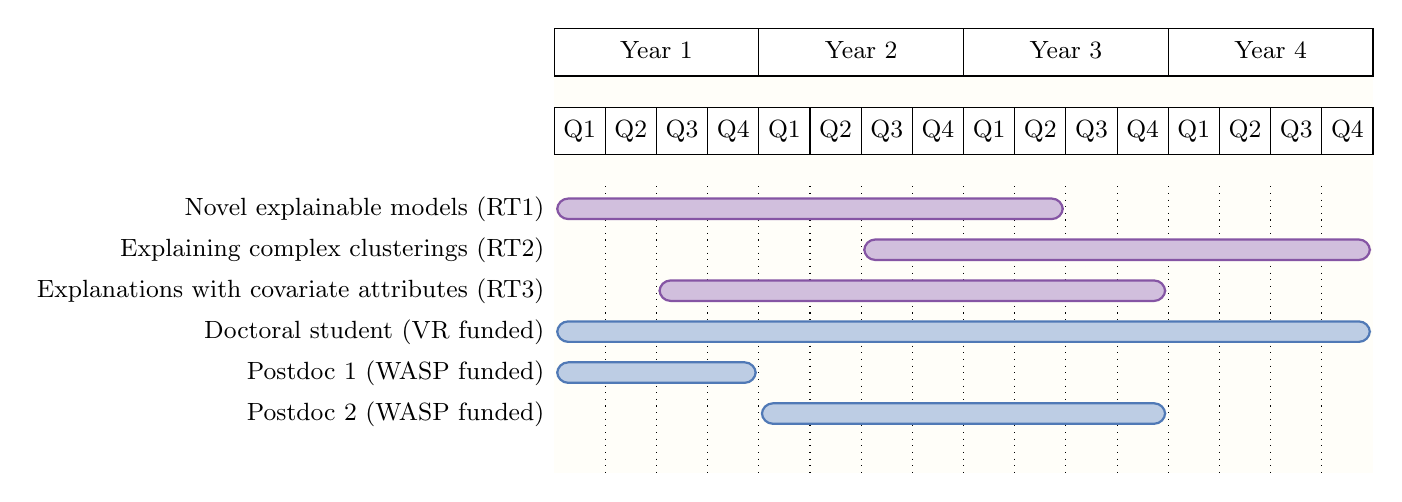
\begin{tikzpicture}
\ganttset{bar height=0.50}
\begin{ganttchart} [
	canvas/.style={fill=yafcolor6!03, very thick},
	x unit=.65cm,
	y unit chart = 0.52cm, 
	hgrid = false,
	vgrid = true, 
	bar right shift=-.06,
	bar left shift=.06,
	milestone/.style={draw=yafcolor3!90,fill=yafcolor3!60, thick}, 
	milestone height = 0.50
]{1}{16}
\gantttitle{\small Year 1}{4} 
\gantttitle{\small Year 2}{4} 
\gantttitle{\small Year 3}{4} 
\gantttitle{\small Year 4}{4} 
\\
% year 1
\gantttitle{\small Q1}{1}
\gantttitle{\small Q2}{1}
\gantttitle{\small Q3}{1}
\gantttitle{\small Q4}{1} 
% year 2
\gantttitle{\small Q1}{1}
\gantttitle{\small Q2}{1}
\gantttitle{\small Q3}{1}
\gantttitle{\small Q4}{1} 
% year 3
\gantttitle{\small Q1}{1}
\gantttitle{\small Q2}{1}
\gantttitle{\small Q3}{1}
\gantttitle{\small Q4}{1} 
% year 4
\gantttitle{\small Q1}{1}
\gantttitle{\small Q2}{1}
\gantttitle{\small Q3}{1}
\gantttitle{\small Q4}{1} 
\\
\ganttbar[bar/.style={rounded corners,inner sep=0pt,thick,draw=yafcolor1!80,fill=yafcolor1!30}]
{\small Novel explainable models (\rto)}{1}{10} \\
\ganttbar[bar/.style={rounded corners,inner sep=0pt,thick,draw=yafcolor1!80,fill=yafcolor1!30}]
{\small Explaining complex clusterings (\rtw)}{7}{16} \\
\ganttbar[bar/.style={rounded corners,inner sep=0pt,thick,draw=yafcolor1!80,fill=yafcolor1!30}]
{\small Explanations with covariate attributes (\rth)}{3}{12} \\

\ganttbar[bar/.style={rounded corners,inner sep=0pt,thick,draw=yafcolor5!80,fill=yafcolor5!30}]
{\small Doctoral student (VR funded)}{1}{16} \\
\ganttbar[bar/.style={rounded corners,inner sep=0pt,thick,draw=yafcolor5!80,fill=yafcolor5!30}]
{\small Postdoc 1 (WASP funded)}{1}{4} \\
\ganttbar[bar/.style={rounded corners,inner sep=0pt,thick,draw=yafcolor5!80,fill=yafcolor5!30}]
{\small Postdoc 2 (WASP funded)}{5}{12} \\
\end{ganttchart}
\end{tikzpicture}


% \begin{ganttchart}[
% 	vgrid,
% 	progress=today,
% 	progress label text=\relax,
% 	today=6
% ]{1}{12}
% \gantttitlecalendar{day} \\[grid]
% \ganttfoobar{Foobar 1}{1}{2} \\
% \ganttfoobar{Foobar 2}{3}{7} \\
% \ganttlinkedfoobar{Foobar 3}{9}{12}
% \end{ganttchart}}
\end{center}
\vspace{-6mm}
\caption{\label{figure:gantt}The time schedule of {\acronym}.}
\vspace{-2mm}
\end{figure}

The time schedule of \acronym is depicted in Figure~\ref{figure:gantt}. 
The diagram shows the duration of the research themes over the life time of the project
and the personnel working on the project.

The funding by the Swedish Research Council will be used to recruit 
one doctoral student who will work exclusively on this project, 
in addition to their teaching duties in KTH.
The PI will allocate 10\% of his time on this project. 
In addition, two postdoctoral researchers in the research team of the PI
will work on the project at 50\% of their time. 
The time of the PI will be funded by his KTH basic funding allocation, 
and the time of the postdocs will be funded by the WASP recruitment package of the PI, 
thus, increasing the added value of this project.
The first postdoctoral researcher is Sebastian Dalleiger, 
who is already a member of the research team, 
while the second postdoc will be recruited in the second year of the project.

In terms of work allocation on the research themes, 
the PI will work on all research themes and will supervise the work of the other team members. 
The doctoral student will work on research themes \#1 and \#2, 
as those are the most closely related and there are many interesting research questions
and ample potential for new methods to develop that fulfill the requirements for a doctoral dissertation. 
The postdocs, together with the PI, will focus on carrying out research theme \#3,
while also helping supervising the doctoral student on themes \#1 and \#2.

\spara{Research output.}
We will aim publishing our work at top-tier international venues, 
focus on quality rather than quantity.
% 
% in the areas of Knowledge Discovery, Machine Learning, and Artificial Intelligence.
% We will focus on the quality of publications rather than quantity.
Target journals 
% for disseminating our work 
are IEEE TKDE, PVLDB, ACM TKDD,  DMKD, etc. 
Target conferences are NeurIPS, ICML, SIGMOD, SIGKDD, WebConf, WSDM, etc.

\spara{Materials.}
Our publications will be available via open access in {\small\url{arxiv.org}}. 
The software and the other outputs of the project 
will become freely available to the scientific community via {\small\url{github.com}}.

\spara{Risks and mitigation.}
Devising efficient algorithms with provable quality guarantees is a challenging task
and the largest risk of the project. 
Achieving this objective, however, offers the largest potential for scientific impact.
%  in the computer science community. 
If we are not able to prove theoretical results, 
we will study problems with simplifying assumptions, and 
will focus on devising heuristic methods and providing thorough empirical validation.
Another risk is recruiting strong team members for the project. 
To mitigate this risk, we will leverage our international network
and the excellent reputation of the research group and research environment in Sweden. 
All the members of the project will be also affiliated with the WASP program, 
which will provide further incentive for recruitment and opportunities 
for network and collaborations during the project.


\subsection{Project organization {\color{orange}[$\approx$0.5 page]} {\color{teal}(Aris)}}

% \instructions{
% Clarify how you and any participating researchers will contribute to the implementation of the project. Explain in particular how the time allocated by you (that is, your activity level) as project leader is suitable for the task, including the relationship with your other research undertakings. Describe and explain the competences and roles of the participating researchers in the project, and also other key persons (including any doctoral students) who are important for the implementation of the project.
% }

The PI will devote 10\% of his time in the project. 
He will supervise the doctoral student and two postdocs, 
be responsible for scientific lead, 
and will allocate time to work on mathematical and algorithmic problems.
He will be responsible for ensuring flow of information and collaborations
with other groups in KTH and his international collaboration network, 
offering the possibility to the group to make research visits and internships.
The PI is currently managing an ERC Advanced Grant (2020 to 2026),
which employs 3 doctoral students and 3 postdocs, 
so the ERC project will be ending during the first year of this project. 
In addition, the PI is still utilizing resources from his WASP recruitment package, 
which are not tied to any specific research project, 
and as explained in the previous section part of those resources will be allocated to the {\acronym} project.

% The doctoral students and postdocs will work in pairs on the corresponding research theme.
For the work in research team, 
we will encourage an environment of openness and collaboration, 
while ensuring that each team member leads their own project.
%
During the hiring process we will support diversity and consider actions to achieve gender balance. 
Currently the PI supervises 6 doctoral students and the gender ratio is 3:3.


% \section{Equipment {\color{orange}[$\approx$0.2 page]} {\color{teal}(Aris)}}

% \instructions{
% Describe the basic equipment you and your team have at your disposal for the project.
% }

\section{Equipment and need for research infrastructure {\color{orange}[$\approx$0.2 page]} {\color{teal}(Aris)}}

% \instructions{
% Specify the project’s need for international and national research infrastructure. If you choose to use other infrastructure than those supported by the Swedish Research Council External link.and that are thereby open to all, you must justify this (also applies to local research infrastructure).
% }

The project is mainly of theoretical nature and will not require extensive computing infrastructure. 
Commodity laptops will be provided to all team members. 
For implementing and evaluating our methods we will use the available 
KTH computing facilities
and the National Academic Infrastructure for Supercomputing in Sweden (NAISS).
The team has also access to the Berzelius supercomputer, 
available to WASP-affiliated faculty, 
which is among the world's 100 fastest AI supercomputers.

\section{International and national collaboration {\color{orange}[$\approx$0.2 page]} {\color{teal}(Aris)}}

% \instructions{
% Describe your own and the team’s collaboration with foreign and Swedish researchers and research teams. State whether you contribute to or refer to international collaboration in your research.
% }

The PI has an extensive international collaboration network. 
Recent and on-going collaborations include
prof.\ De Bie in Ghent University, 
prof.\ Terzi in Boston University,
prof.\ Mannila in Aalto University, and 
Dr.\ Bonchi in Centai Labs.
In spring 2024 the PI will spent one month as a visiting professor 
in Sapienza University of Rome, hosted by prof.\ Leonardi.
In the near future the PI will apply for a sabbatical in Stanford University, 
planning to visit prof.\ Ugander. 
We will seek to strengthen and further expand this collaboration network.
We will encourage the research team to be actively involved in national and international collaborations
and make research visits and internships in other institutes.

\section{Independent line of research {\color{orange}[$\approx$0.2 page]} {\color{teal}(Aris)}}

\instructions{
If you are working or will be working in a larger group, please clarify how your project relates to the other projects in the group. If you are (continuing) working in the same team as your doctoral or postdoc supervisor, or if you are continuing a project that wholly or partly started during your doctoral or postdoc studies, you must also describe the relationship between your project and the research of your former supervisor.
}



{\small
\setlength{\bibsep}{0pt}
\bibliographystyle{abbrv}
\bibliography{references}
}

{\color{orange}References 1 page maximum} 

% \newpage
% \input{rebound}

\end{document}




